\chead{\textit{Application}}  				
\section{Application}


\subsection{Modeling Framework}

This section introduces the reader to all relevant information about the modelling framework that is used to model a real-life application. The modelling framework has to cover certain requirements. Firstly, there should be generators that produce electrical power. The power output is only limited by the maximum capacity of the generator. There exist no ramping constraints or minimum up- and down-times. Each generator has marginal costs and is connected to a specific node. To depict these requirements in Julia, a generator structure was implemented as you can see in the following code snippet. In addition to the stated requirements, the structure also contains a colour and a name. These attributes are mainly used for evaluation reasons and are not important for modelling purposes. 

\lstinputlisting[language=julia, firstline=7, lastline=13, caption=Julia structure for node element]{../src/structures/network_elements.jl}

Another part of the modelling framework is a storage unit. Storages should be able to store a surplus of energy as well as deliver electrical power by discharging their capacity. The power input or output is also limited by a maximum value. In addition, a storage unit should only be able to store a certain amount of energy. This is depicted by the storage level. As generators, storages have specific marginal costs for charging and discharging and are connected to a specific node. A Julia structure was implemented respectively.  

As written before, generators and storages are located at network nodes. These nodes have a specific demand that should be matched by the output of the generating units. For modelling purposes, it is also crucial to define a slack node to compensate the power flow balance. The node structure was implemented as follows:

\lstinputlisting[language=julia, firstline=1, lastline=5, caption=Julia structure for generator element]{../src/structures/network_elements.jl}

The last element of the framework is a transmission line. This element connects nodes and enables the exchange of energy. Transmission lines are characterized by their maximum capacity and their susceptance value. However, susceptance might not be the correct term here since the model does not consider alternating current. Thus, the correct name would be conductance but is not used to follow general naming conventions. A Julia structure was also implemented for this network element.

Lastly, the modelling framework has to consider multi-periods. This is crucial since without multi periods, it would not make sense to include storages into the system.

 
\subsection{Three Node System}

The following section describes the \gls{tns} which will be used throughout the chapter to explain the optimization models and to derive the corresponding equations. The system consists of three nodes. At each of them, a different set of generators and storages is located and a multi-period load curve exists. To simplify the equations, only two time steps are considered. The nodes are connected by a total of three transmission lines. Thus, every node has two neighbours. Figure (\ref{fig:tns}) illustrates the described system.

%TODO Make own graphic for three node system
\begin{figure}[h]
	\centering
	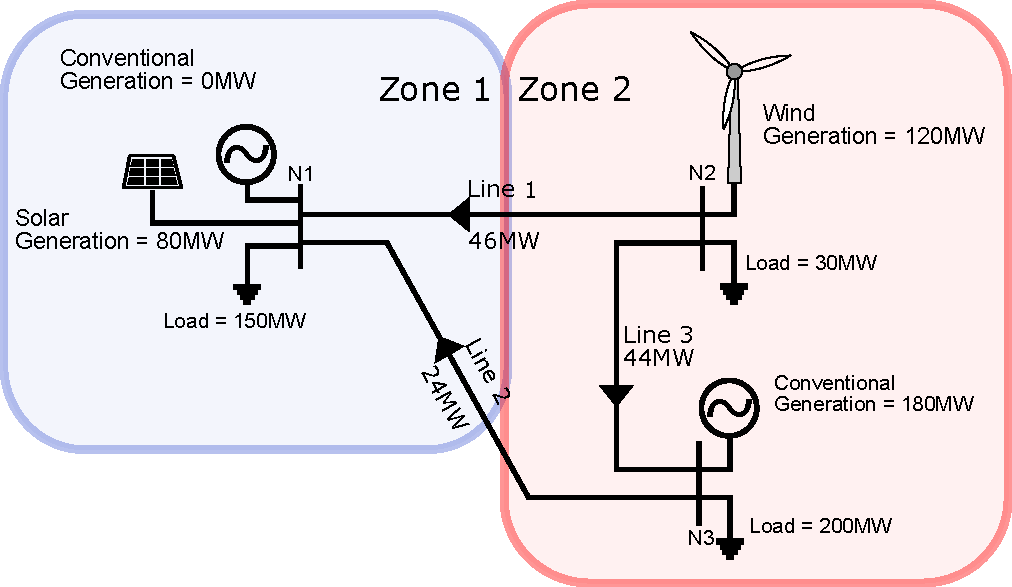
\includegraphics[width=0.8\textwidth]{three-node-system.png}
	\caption{Exemplary Three Node System}
	\label{fig:tns}
\end{figure}

\subsection{Problem formulations}

\subsubsection{General problem}
\label{sec:general_formulation}

The following optimization problem describes a basic economic dispatch with network restrictions.

\begin{subequations}
	\begin{align}
		 \min \quad & \sum_{t\in\mathcal{T}}\sum_{g\in\mathcal{G}}c_g*P_g(t) + \sum_{s\in\mathcal{S}}c_s*(P_s^d(t)+P_s^c(t))\\
		 \text{s.t. } \quad & 0 \leq P_g(t) \leq \overline{P_g} && \forall g \in \set{G}, t \in \set{T}\\
		 & 0 \leq P_s^d(t) \leq \overline{P_s} && \forall s \in \set{S}, t \in \set{T}\\
		 & 0 \leq P_s^c(t) \leq \overline{P_s} && \forall s \in \set{S}, t \in \set{T}\\
		 & 0 \leq E_s(t) \leq \overline{E_s} && \forall s \in \set{S}, t \in \set{T}\\
		 & E_s(t) - E_s(t-1) - P_s^c(t) + P_s^d(t) = 0 && \forall s \in \set{S}, t \in \set{T}\\
		 & I_n(t) = \sum_{g\in\mathcal{G}}P_g(t) + \sum_{s\in\mathcal{S}}(P_s^d(t)-P_s^c(t))-D_n(t) = 0 && \forall t \in \set{T}, n \in \set{N}\\
		 & -\overline{L_l} \leq PTDF * I_n(t) \leq \overline{L_l} && \forall l \in \set{L}, t \in \set{T}, n \in \set{N} \label{eq:con_power_flow_all}
	\end{align}
\end{subequations}

\subsubsection{Replace inequality line constraint}

Since the \gls{admm} can not cope with inequality constraints, equation (\ref{eq:con_power_flow_all}) is replaced by two equality constraints by introducing two slack variables $R_{ref}$ and $R_{cref}$. The problem formulation evolves to the following:

\begin{subequations}
	\begin{align}
		 \min \quad & \sum_{t\in\mathcal{T}}\sum_{g\in\mathcal{G}}c_g*P_g(t) + \sum_{s\in\mathcal{S}}c_s*(P_s^d(t)+P_s^c(t))\\
		 \text{s.t. } \quad & 0 \leq P_g(t) \leq \overline{P_g} && \forall g \in \set{G}, t \in \set{T}\\\
		 & 0 \leq P_s^d(t) \leq \overline{P_s} && \forall s \in \set{S}, t \in \set{T}\\
		 & 0 \leq P_s^c(t) \leq \overline{P_s} && \forall s \in \set{S}, t \in \set{T}\\
		 & 0 \leq E_s(t) \leq \overline{E_s} && \forall s \in \set{S}, t \in \set{T}\\
		 & E_s(t) - E_s(t-1) - P_s^c(t) + P_s^d(t) = 0 && \forall s \in \set{S}, t \in \set{T}\\
		 & I_n(t) = \sum_{g\in\mathcal{G}}P_g(t) + \sum_{s\in\mathcal{S}}(P_s^d(t)-P_s^c(t))-D_n(t) = 0 && \forall t \in \set{T}, n \in \set{N} \label{eq:con_energy_balance}\\
		 & PTDF * I_n(t) + R_{ref} - \overline{L_l} = 0 && \forall l \in \set{L}, t \in \set{T}, n \in \set{N} \label{eq:con_power_flow_upper} \\
		 & R_{cref} - PTDF * I_n(t) - \overline{L_l} = 0 && \forall l \in \set{L}, t \in \set{T}, n \in \set{N} \label{eq:con_power_flow_lower}
	\end{align}
\end{subequations}

The complicating constraints are equations (\ref{eq:con_energy_balance}), (\ref{eq:con_power_flow_upper}) and (\ref{eq:con_power_flow_lower}). If these constraints are relaxed, the main problem decomposes into a generator and a storage subproblem.

\subsubsection{Augmented Lagrangian Relaxation}

The complicated constraints are relaxed by implementing a max-min problem using the dual variables of the complicated constraints. Hereby, $\lambda$ is the dual of the energy balance constraint, $\mu$ and $\rho$ are the duals of the upper and lower flow constraint respectively. Since the objective function is linear, the relaxation is implemented by using the \gls{alr}. Thus, a penalty term per dual variable is added whose value equals zero in the optimality point. 

\begin{subequations}
	\begin{align}
		\max{(\lambda, \mu, \rho)}\\
		 & \min{(P_\mathcal{G}, P_\mathcal{S}^d, P_\mathcal{S}^c)} \quad \sum_{t\in\mathcal{T}}\sum_{g\in\mathcal{G}}c_g*P_g(t) + \sum_{s\in\mathcal{S}}c_s*(P_s^d(t)+P_s^c(t)) \nonumber \\
		 & + \lambda * \left[\sum_{g\in\mathcal{G}}P_g(t) + \sum_{s\in\mathcal{S}}(P_s^d(t)-P_s^c(t))-D_n(t))\right]\nonumber \\
		 & + \frac{\gamma}{2} * \bigg\|\sum_{g\in\mathcal{G}}P_g(t) + \sum_{s\in\mathcal{S}}(P_s^d(t)-P_s^c(t))-D_n(t))\bigg\|_2^2 \nonumber \\
		 & + \mu * \left[PTDF * I_n(t) + R_{ref} - \overline{L_l}\right] \nonumber \\
		 & + \frac{\gamma}{2} * \bigg\|PTDF * I_n(t) + R_{ref} - \overline{L_l}\bigg\|_2^2 \nonumber \\
		 & + \rho * \left[R_{cref} - PTDF * I_n(t) - \overline{L_l}\right]\nonumber \\
		 & + \frac{\gamma}{2} * \bigg\|R_{cref} - PTDF * I_n(t) - \overline{L_l}\bigg\|_2^2\nonumber
	\end{align}
	\begin{align}
		 \text{s.t. } \quad & 0 \leq P_g(t) \leq \overline{P_g} && \forall g \in \set{G}, t \in \set{T}\\\
		 & 0 \leq P_s^d(t) \leq \overline{P_s} && \forall s \in \set{S}, t \in \set{T}\\
		 & 0 \leq P_s^c(t) \leq \overline{P_s} && \forall s \in \set{S}, t \in \set{T}\\
		 & 0 \leq E_s(t) \leq \overline{E_s} && \forall s \in \set{S}, t \in \set{T}\\
		 & E_s(t) - E_s(t-1) - P_s^c(t) + P_s^d(t) = 0 && \forall s \in \set{S}, t \in \set{T}
	\end{align}
\end{subequations}

\subsubsection{Matrix Form}

Typically, \gls{admm} solves problems in the form:

\begin{subequations}
	\begin{align}
		\min{(x, z)} \quad & f(x) + g(z) \\
		\text{s.t. } \quad & \vb{A}x + \vb{B}z = c
	\end{align}
\end{subequations}

If applied to the formulation in the section \ref{sec:general_formulation}, the generator problem looks like:

\begin{subequations}
	\begin{align}
		f(x) &= f(\vb{P_\mathcal{G}}) = \vb{P_\mathcal{G}}^T * \va{c_\mathcal{G}}\\
		& = \begin{bmatrix}
			P_{g_1}(t_1) & P_{g_2}(t_1) & P_{g_3}(t_1) \\
			P_{g_1}(t_2) & P_{g_2}(t_2) & P_{g_3}(t_2)
		\end{bmatrix} * \begin{bmatrix}
			c_{g_1} \\
			c_{g_2} \\
			c_{g_3}
		\end{bmatrix} \\
		& = \begin{bmatrix}
			P_{g_1}(t_1) * c_{g_1} + P_{g_2}(t_1) * c_{g_2} + P_{g_3}(t_1) * c_{g_3} \\
			P_{g_1}(t_2) * c_{g_1} + P_{g_2}(t_2) * c_{g_2} + P_{g_3}(t_2) * c_{g_3} \\
		\end{bmatrix}
	\end{align}
\end{subequations}

In addition, the storage problem yields:

\begin{subequations}
	\begin{align}
		g(z) &= g(\vb{P_\mathcal{S}^d}, \vb{P_\mathcal{S}^c})\\
		& = \left(\vb{P_\mathcal{S}^d}^T + \vb{P_\mathcal{S}^c}^T\right) * \va{c_\mathcal{S}} \\
		& = \left(\begin{bmatrix}
			P_{s_1}^d(t_1) & P_{s_2}^d(t_1) \\
			P_{s_1}^d(t_2) & P_{s_2}^d(t_2)
		\end{bmatrix} + \begin{bmatrix}
			P_{s_1}^c(t_1) & P_{s_2}^c(t_1) \\
			P_{s_1}^c(t_2) & P_{s_2}^c(t_2)
		\end{bmatrix} \right) * \begin{bmatrix}
			c_{s_1} \\
			c_{s_2}
		\end{bmatrix} \\
		& = \begin{bmatrix}
			P_{s_1}^d(t_1) + P_{s_1}^c(t_1) & P_{s_2}^d(t_1) + P_{s_2}^c(t_1) \\
			P_{s_1}^d(t_2) + P_{s_1}^c(t_2) & P_{s_2}^d(t_2) + P_{s_2}^c(t_2)
		\end{bmatrix} * \begin{bmatrix}
			c_{s_1} \\
			c_{s_2}
		\end{bmatrix} \\
		& = \begin{bmatrix}
			P_{s_1}(t_1) * c_{s_1} + P_{s_2}(t_1) * c_{s_2} \\
			P_{s_1}(t_2) * c_{s_1} + P_{s_2}(t_2) * c_{s_2} \\
		\end{bmatrix}
	\end{align}
\end{subequations}

Only the energy balance constraint and the constraints for the power flow are part of the \gls{admm} formulation. All the other constraints are either part of the generator problem or of the storage problem and can be easily decomposed. \\

For this example, only generator 2 and storage 2 are located at node 2. The other resources are located at node 1. Then, the energy balance constraint in matrix form yields:

\begin{subequations}
	\begin{align}
		& \vb{N_\mathcal{G}}*\vb{P_\mathcal{G}} + \vb{N_\mathcal{S}}*(\vb{P_\mathcal{S}^d} - \vb{P_\mathcal{S}^c}) - \vb{D_\mathcal{N}} = \vb{I_\mathcal{N}} = \vb{0} \\
		& \Leftrightarrow \begin{bmatrix}
			1 & 0 & 1 \\
			0 & 1 & 0 \\
		\end{bmatrix} * \begin{bmatrix}
				P_{g_1}(t_1) & P_{g_1}(t_2) \\
				P_{g_2}(t_1) & P_{g_2}(t_2) \\
				P_{g_3}(t_1) & P_{g_3}(t_2)
		\end{bmatrix} \\
		& \qquad + \begin{bmatrix}
			1 & 0 \\
			0 & 1 \\
		\end{bmatrix} * \left(\begin{bmatrix}
			P_{s_1}^d(t_1) & P_{s_1}^d(t_2) \\
			P_{s_2}^d(t_1) & P_{s_2}^d(t_2)
		\end{bmatrix} - \begin{bmatrix}
			P_{s_1}^c(t_1) & P_{s_1}^c(t_2) \\
			P_{s_2}^c(t_1) & P_{s_2}^c(t_2)
		\end{bmatrix} \right) \nonumber \\
		& \qquad - \begin{bmatrix}
			D_{n_1}(t_1) & D_{n_1}(t_2) \\
			D_{n_2}(t_1) & D_{n_2}(t_2)
		\end{bmatrix} = \begin{bmatrix}
			0 & 0 \\
			0 & 0
		\end{bmatrix} \nonumber \\
		& \Leftrightarrow \begin{bmatrix}
				P_{g_1}(t_1) + P_{g_3}(t_1) & P_{g_1}(t_2) + P_{g_3}(t_2) \\
				P_{g_2}(t_1) & P_{g_2}(t_2)
		\end{bmatrix} + \begin{bmatrix}
			P_{s_1}^d(t_1) - P_{s_1}^c(t_1) & P_{s_1}^d(t_2) - P_{s_1}^c(t_2) \\
			P_{s_2}^d(t_1) - P_{s_2}^c(t_1) & P_{s_2}^d(t_2) - P_{s_2}^c(t_2)
		\end{bmatrix} \nonumber \\
		& \qquad - \begin{bmatrix}
			D_{n_1}(t_1) & D_{n_1}(t_2) \\
			D_{n_2}(t_1) & D_{n_2}(t_2)
		\end{bmatrix} = \begin{bmatrix}
			0 & 0 \\
			0 & 0
		\end{bmatrix} \nonumber \\
		& \Leftrightarrow \begin{bmatrix}
			P_{g_1}(t_1) + P_{g_3}(t_1) + P_{s_1}^d(t_1) - P_{s_1}^c(t_1) - D_{n_1}(t_1) & P_{g_1}(t_2) + P_{g_3}(t_2) + P_{s_1}^d(t_2) - P_{s_1}^c(t_2) - D_{n_1}(t_2) \\
			P_{g_2}(t_1) + P_{s_2}^d(t_1) - P_{s_2}^c(t_1) - D_{n_2}(t_1) & P_{g_2}(t_2) + P_{s_2}^d(t_2) - P_{s_2}^c(t_2) - D_{n_2}(t_2)
		\end{bmatrix} \\
		& \qquad = \begin{bmatrix}
			0 & 0 \\
			0 & 0
		\end{bmatrix} \nonumber
	\end{align}
\end{subequations}

The power flow constraints are set up accordingly. The \gls{admm} formulation becomes:

\begin{subequations}
	\begin{align}
		\max{(\lambda, \mu, \rho)} \label{eq:opt_admm_matrix}\\
		 & \min{(\vb{P_\mathcal{G}}, \vb{P_\mathcal{S}^d}, \vb{P_\mathcal{S}^c})} \quad \vb{P_\mathcal{G}}^T * \va{c_\mathcal{G}} + \left(\vb{P_S^d} + \vb{P_S^c}\right)^T * \va{c_\mathcal{S}} \nonumber \\
		 & + \vb{\lambda} * \vb{I_\mathcal{N}} + \frac{\gamma}{2} * \big\|\vb{I_\mathcal{N}}\big\|_2^2 \nonumber \\
		 & + \vb{\mu} * \left[ PTDF * \vb{I_\mathcal{N}} + \vb{R_\mathcal{L}^{ref}} - \vb{\overline{L_\mathcal{L}}} \right] \nonumber \\
		 & + \frac{\gamma}{2} * \big\| PTDF * \vb{I_\mathcal{N}} + \vb{R_\mathcal{L}^{ref}} - \vb{\overline{L_\mathcal{L}}} \big\|_2^2 \nonumber \\
		 & + \vb{\rho} * \left[ \vb{R_\mathcal{L}^{cref}} - PTDF * \vb{I_\mathcal{N}} - \vb{\overline{L_\mathcal{L}}} \right] \nonumber \\
		 & + \frac{\gamma}{2} * \big\| \vb{R_\mathcal{L}^{cref}} - PTDF * \vb{I_\mathcal{N}} - \vb{\overline{L_\mathcal{L}}} \big\|_2^2 \nonumber
	\end{align}
		\begin{align}
		 \text{s.t. } \quad & \vb{0} \leq \vb{P_\mathcal{G}} \leq \vb{\overline{P_\mathcal{G}}} \\
		 & \vb{0} \leq \vb{P_\mathcal{S}^d} \leq \vb{\overline{P_\mathcal{S}}} \\
		 & \vb{0} \leq \vb{P_\mathcal{S}^c} \leq \vb{\overline{P_\mathcal{S}}} \\
		 & \vb{0} \leq \vb{E_\mathcal{S}} \leq \vb{\overline{E_\mathcal{S}}}\\
		 & \vb{0} = \vb{E_\mathcal{S}} - \vb{E_\mathcal{S}^{t-1}} - \vb{P_\mathcal{S}^c} + \vb{P_\mathcal{S}^d}
	\end{align}
\end{subequations}

\subsubsection{Scaled Form}

According to \citet{Boyd-2010-DistributedOptimizationStatistical}, \gls{admm} is often written in a shorter, so called scaled form. In this form, the linear and quadratic terms of the objective function are combined and the dual variables are scaled. This yields a much shorter formulation. As an example, the scaled dual variable of the energy balance is derived. First, one defines a residual term of the energy balance constraint.

\begin{equation}
	\vb{r} = \vb{N_\mathcal{G}}*\vb{P_\mathcal{G}} + \vb{N_\mathcal{S}}*(\vb{P_\mathcal{S}^d} - \vb{P_\mathcal{S}^c}) - \vb{D_\mathcal{N}} = \vb{I_\mathcal{N}}
\end{equation}

%Respectively, one can also define the residuals for the power flow constraints.
%
%\begin{equation}
%	\vb{s} = PTDF * \vb{I_\mathcal{N}} + \vb{R_\mathcal{L}^{ref}} - \vb{\overline{L_\mathcal{L}}}
%\end{equation} 
%\begin{equation}
%	\vb{t} = \vb{R_\mathcal{L}^{cref}} - PTDF * \vb{I_\mathcal{N}} - \vb{\overline{L_\mathcal{L}}}
%\end{equation}

Inserting the residual term into the corresponding part of the optimization problem yields:

\begin{equation}
	\vb{\lambda} * \vb{r} + \frac{\gamma}{2} * || \vb{r} ||^2_2 = \frac{\gamma}{2} || \vb{r} + \frac{1}{\gamma}\vb{\lambda} ||^2_2 - \frac{1}{2\gamma}|| \vb{\lambda} ||^2_2 = \frac{\gamma}{2} || \vb{r} + \vb{\hat{\lambda}} ||^2_2 - \frac{\gamma}{2}|| \vb{\hat{\lambda}} ||^2_2 \label{eq:derivation_lambda_hat}
\end{equation}

The transformation is not very straight forward but allows to further simplify the main optimization problem in equation (\ref{eq:opt_admm_matrix}). With $\vb{\hat{\lambda}} = \frac{1}{\gamma}*\vb{\lambda}$, one gets the scaled dual variable of $\vb{\lambda}$. Using the scaled dual variable makes the problem formulation much shorter because the last term $- \frac{\gamma}{2}|| \vb{\hat{\lambda}} ||^2_2$ of equation (\ref{eq:derivation_lambda_hat}) does not contain any optimization variable. Hence, this term can be removed. The other dual variables can be replaced respectively. Inserting all scaled dual variables $\vb{\hat{\lambda}}$, $\vb{\hat{\mu}}$, $\vb{\hat{\rho}}$ in equation (\ref{eq:opt_admm_matrix}) yields:

\begin{subequations}
	\begin{align}
		\max{(\lambda, \mu, \rho)} \label{eq:opt_admm_matrix_scaled}\\
		 & \min{(\vb{P_\mathcal{G}}, \vb{P_\mathcal{S}^d}, \vb{P_\mathcal{S}^c})} \quad \vb{P_\mathcal{G}}^T * \va{c_\mathcal{G}} + \left(\vb{P_S^d} + \vb{P_S^c}\right)^T * \va{c_\mathcal{S}} \nonumber \\
		 & + \frac{\gamma}{2} * \big\|\vb{I_\mathcal{N}} + \vb{\hat{\lambda}}\big\|_2^2 \nonumber \\
		 & + \frac{\gamma}{2} * \big\| PTDF * \vb{I_\mathcal{N}} + \vb{R_\mathcal{L}^{ref}} - \vb{\overline{L_\mathcal{L}}} + \vb{\hat{\mu}} \big\|_2^2 \nonumber \\
		 & + \frac{\gamma}{2} * \big\| \vb{R_\mathcal{L}^{cref}} - PTDF * \vb{I_\mathcal{N}} - \vb{\overline{L_\mathcal{L}}} + \vb{\hat{\rho}} \big\|_2^2 \nonumber
	\end{align}
		\begin{align}
		 \text{s.t. } \quad & \vb{0} \leq \vb{P_\mathcal{G}} \leq \vb{\overline{P_\mathcal{G}}} \\
		 & \vb{0} \leq \vb{P_\mathcal{S}^d} \leq \vb{\overline{P_\mathcal{S}}} \\
		 & \vb{0} \leq \vb{P_\mathcal{S}^c} \leq \vb{\overline{P_\mathcal{S}}} \\
		 & \vb{0} \leq \vb{E_\mathcal{S}} \leq \vb{\overline{E_\mathcal{S}}}\\
		 & \vb{0} = \vb{E_\mathcal{S}} - \vb{E_\mathcal{S}^{t-1}} - \vb{P_\mathcal{S}^c} + \vb{P_\mathcal{S}^d}
	\end{align}
\end{subequations}

The scaled dual variables can be again replaced by the dual variable. \textbf{Maybe that is better to be more consistent.}
